\documentclass[xcolor=svgnames]{beamer}
\usepackage{multirow,textcomp,color}
\usepackage{rotating}
\usepackage{amssymb,amsfonts,amsmath}
\usepackage{mathptmx,bm}
\usepackage{epsfig}

% Find colour names http://calque.pagesperso-orange.fr/latex/latexps.html
%[xcolor=dvipsnames]

\usecolortheme[named=DarkBlue]{structure} % colour from svgnames
%\usecolortheme[named=Gray]{structure} % colour from svgnames
%\usecolortheme[named=LightGray]{structure} % colour from svgnames
%\usecolortheme[named=LightBlue]{structure} % colour from svgnames
%\usecolortheme[named=Teal]{structure} % colour from svgnames
%\usecolortheme[named=OliveGreen]{structure} % colour from dvipsnames
%\usefonttheme{serif}
%\usetheme{Rochester}
\usetheme{Singapore}
\setbeamertemplate{footline}[frame number]
%\setbeamercolor{frametitle}{fg=DarkBlue,bg=Tan}
%\setbeamercolor{title}{fg=DarkRed,bg=LightGray}
%\setbeamercolor{title}{fg=Navy,bg=Wheat}
\setbeamerfont{frametitle}{size=\Large,series=\bfseries}
\setbeamerfont{title}{size=\Large,series=\bfseries}

\begin{document}
%%%%%%%%%%%%%%%%%%%%%%%%%%%%%%%%%%%%%%%%%%%%%%%%%%%%%%%%%%%%%%%%%%%%%%%%%%%%%
\title{Cluster prediction by statistical modeling for Ordinal Data}
\author{Quan Zhao ({\tt felixz2010@gmail.com})\\[1em]
{\em student id: 300471028}\\[1em]
}

\date{2024}

%-----------------------------------------------------------------------------

\begin{frame}\frametitle{
}
\titlepage
\end{frame}

%-----------------------------------------------------------------------------

\begin{frame}\frametitle{Outline}

\begin{enumerate}
\item Introduction
\begin{itemize}
\item Ordinal data
\item Clustering
\item Finite Mixture Models
\end{itemize}
\item Methods
\item Research Goals
\end{enumerate}

\end{frame}
%-----------------------------------------------------------------------------

\begin{frame}\frametitle{Background: Ordinal data}

{\bf The response variable has ordinal categorical scales}

Ordinal data is widely used in areas such as marketing, social, medical and ecological science.

\begin{itemize}
\pause
\item  \textcolor{blue}{Likert scale}:  ``strongly disagree'', ``disagree'', ``agree'', or ``strongly agree'' in a survey.
\pause
\item \textcolor{blue}{Braun-Blanquet cover-abundance scale} is very common in vegetation analysis. 
\end{itemize}

\end{frame}


%-----------------------------------------------------------------------------
\begin{frame}\frametitle{Background: Ordinal data}

\begin{itemize}
 \item 
Data represented as a matrix $Y$ with dimensions $n\times m$ ($n$ could be species., $m$ could be sites) where
  \begin{equation*} 
      y_{ij} \in \{1,\ldots,q\} \hspace{25pt} i=1,\ldots,n \hspace{15pt} j=1,\ldots,m \hspace{15pt} q\;categories.
  \end{equation*}
\pause
  \item \color{black}{For example, Spider data: }
      \begin{itemize}
	\scriptsize
	\item $n=12$ species (rows)
	\item $m=28$ sites (columns).
	\item $q=4$ categories: Absence (0),\\ \hspace{2cm} Presences: (0,25\%] (1), (25,65\%] (2) and (65,100\%] (3)
\pause
      \end{itemize}
\vspace*{-0.5in}
\begin{minipage}{0.6\textwidth}{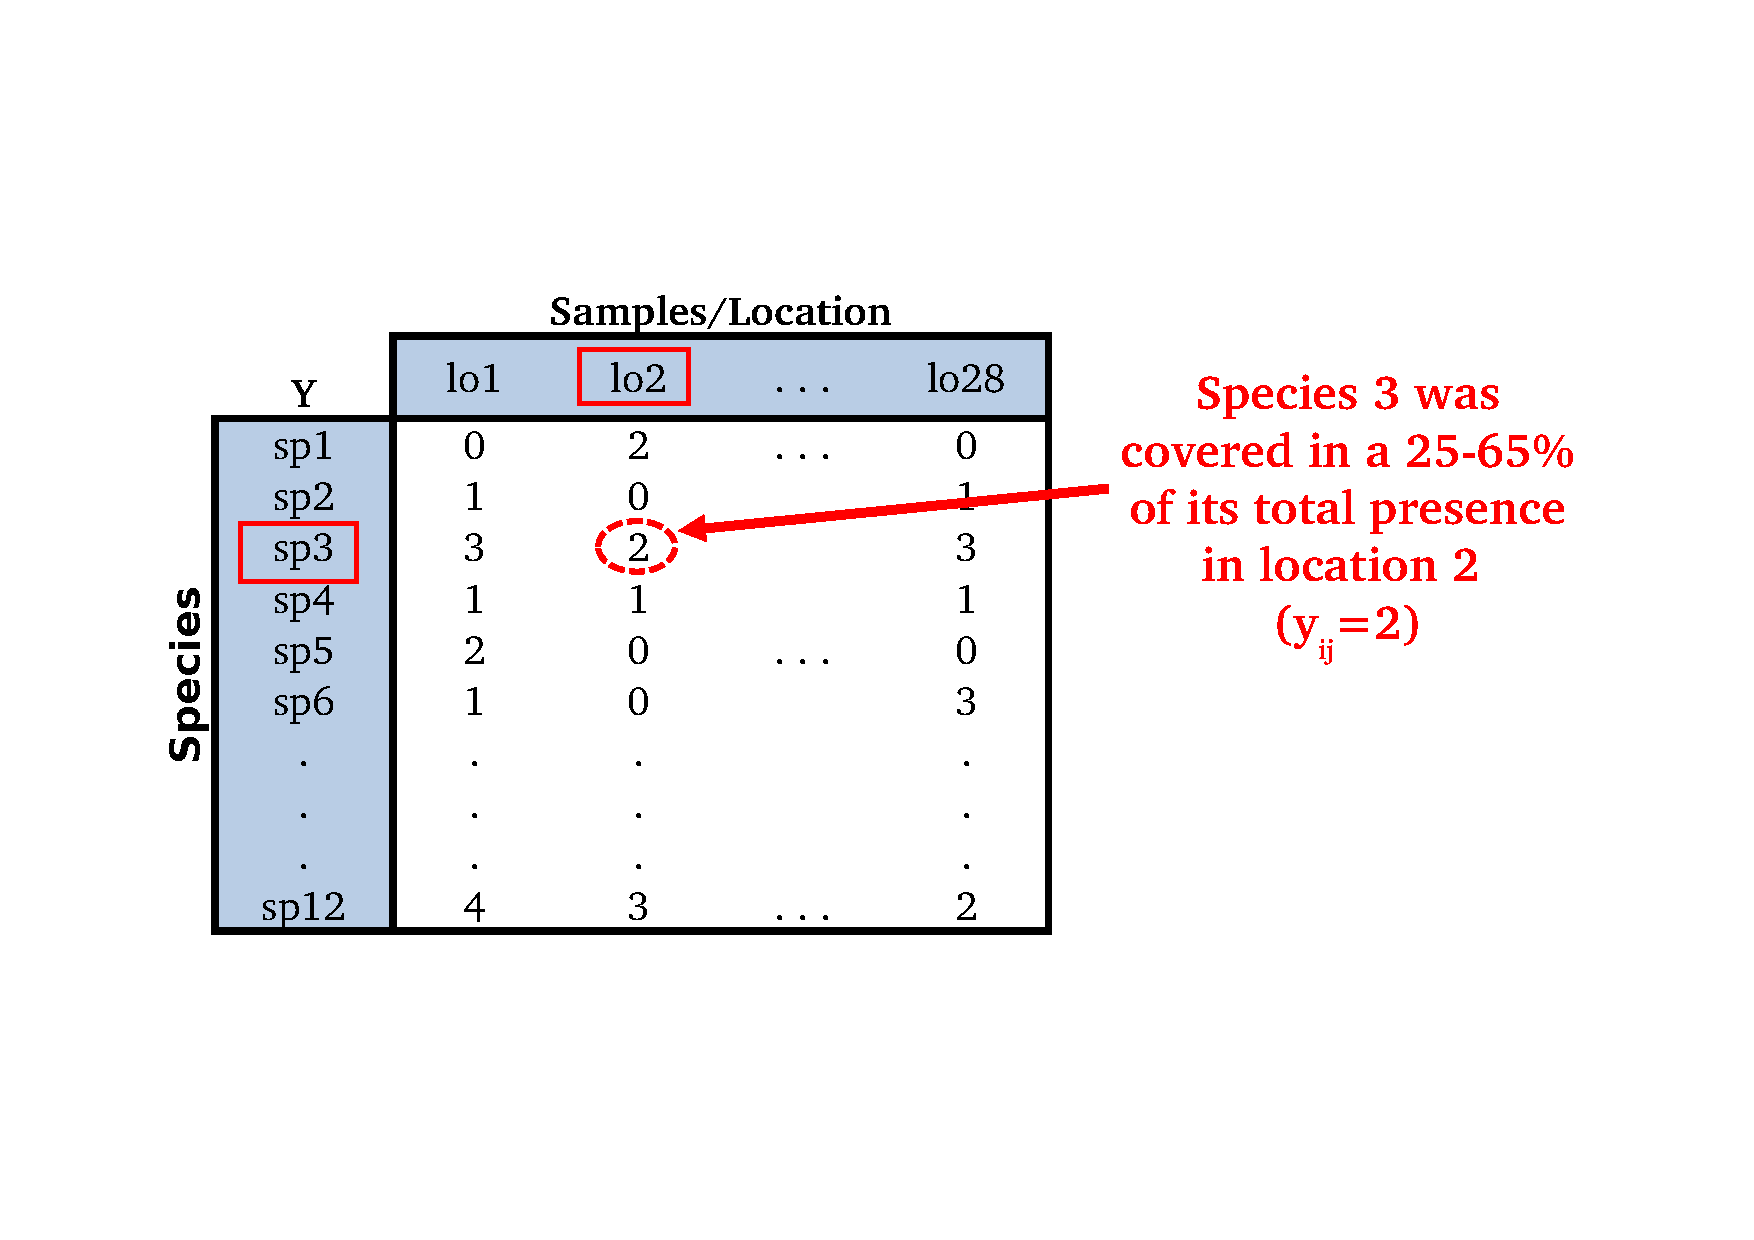
\epsfig{file=images/datamatrix_spider.pdf,width=1.3\linewidth}}\end{minipage}
\end{itemize}

\end{frame}
%--------------------------------------------------------
\begin{frame}\frametitle{Background: Proportional odds model}

Now, consider $Y$ has $c$ ordered categories.  For instance, let $c=3$ ( 1=''worse'', 2=''unchanged'', 3=''better'').

\pause
\begin{minipage}{0.5\textwidth}{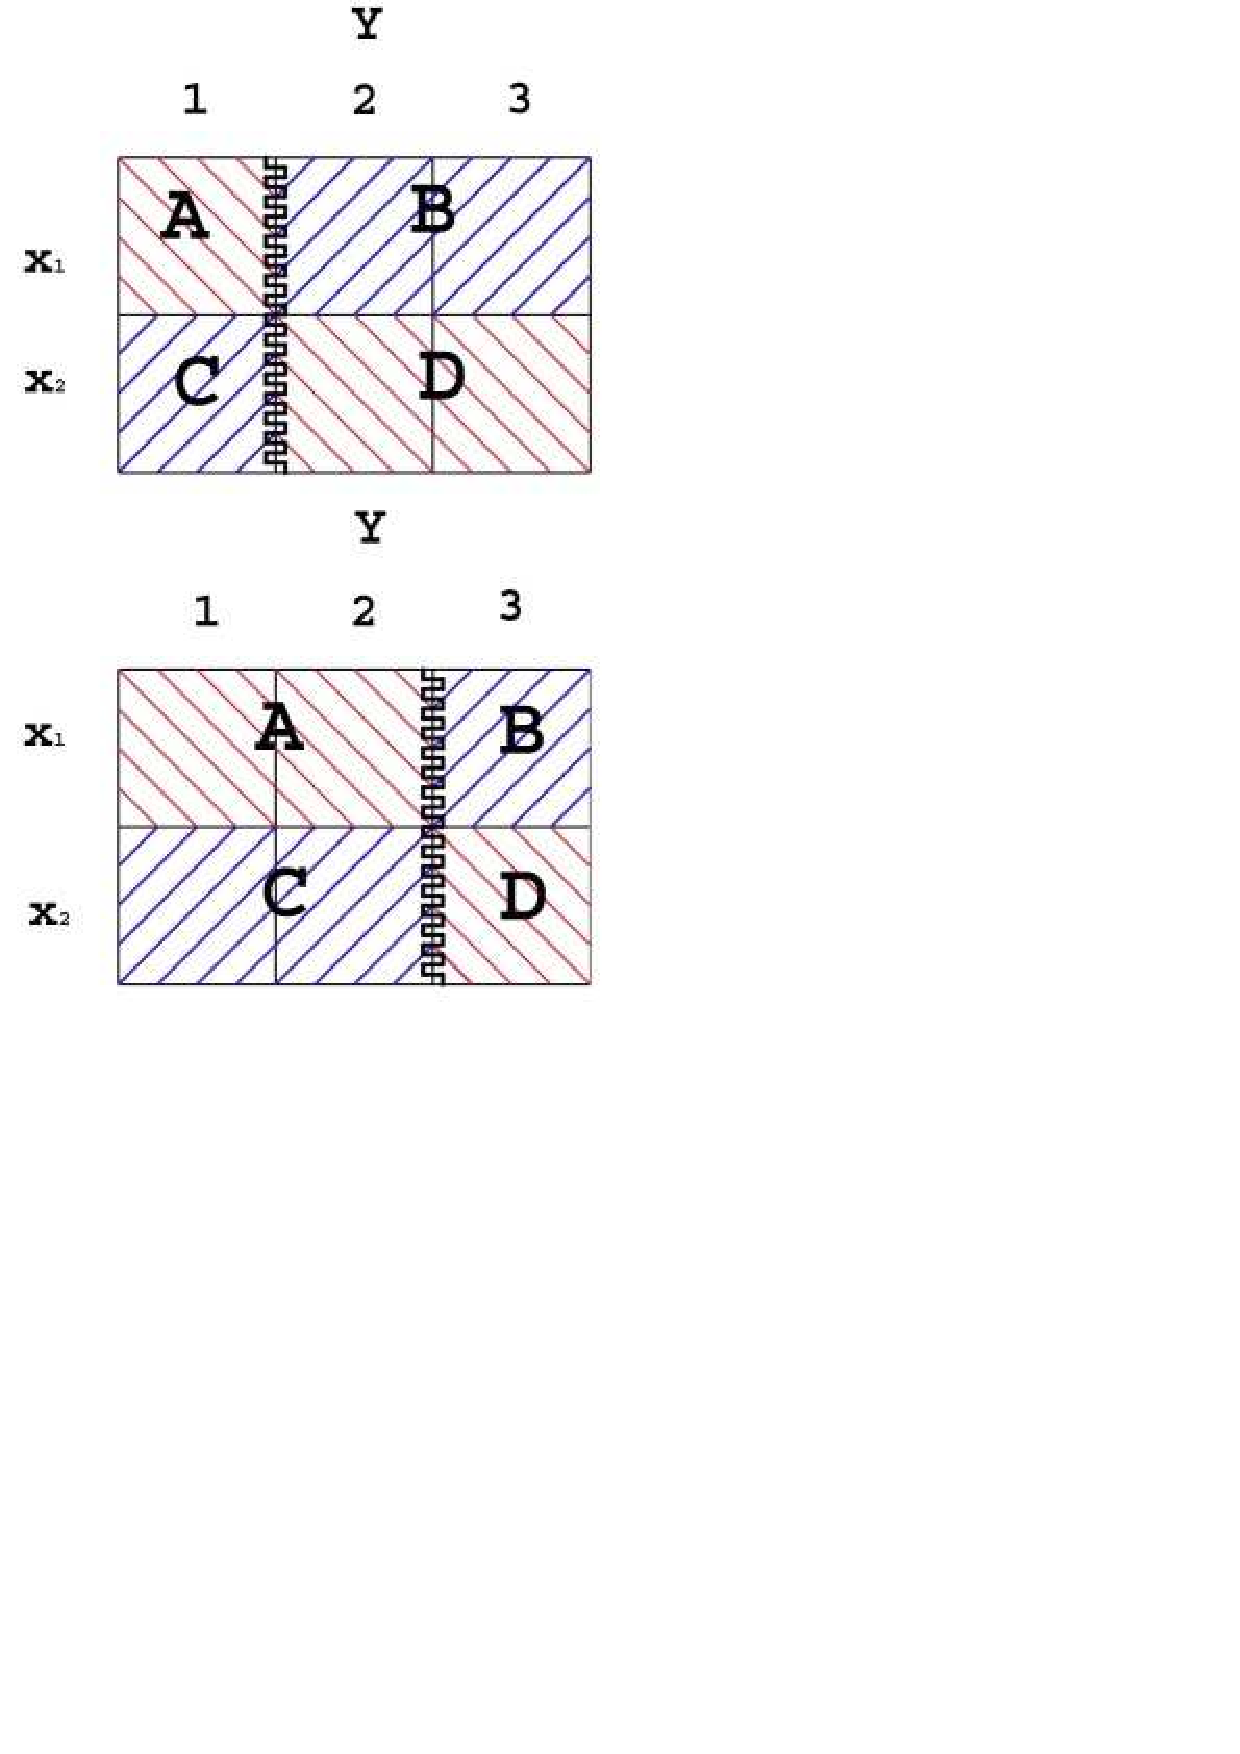
\epsfig{file=images/Pic2.pdf,width=1.3\linewidth}}\end{minipage}
\begin{minipage}{0.45\textwidth}{\vspace{-1.5in}There are $c-1$  possible ways of collapsing a $c$-category response to a binary variable.\vspace{.2in}  \\  The proportional odds model implies that the odds
ratios ($=\frac{A\times D}{B\times C}$) for describing effects of $X$ on the response variable are the same for each of these tables.
}\end{minipage}
\end{frame}
%--------------------------------------------------------

\end{document}
